\documentclass[tikz]{standalone}

\usepackage{cmap}%allows cyrillic search in pdf
\usepackage[english,russian,ukrainian]{babel}
\usepackage[T2A]{fontenc}
\usepackage[utf8]{inputenc}
\usepackage{graphics,overpic}

\begin{document}
\begin{tikzpicture}
            \node[anchor=south west,inner sep=0] (image) at (0,0) {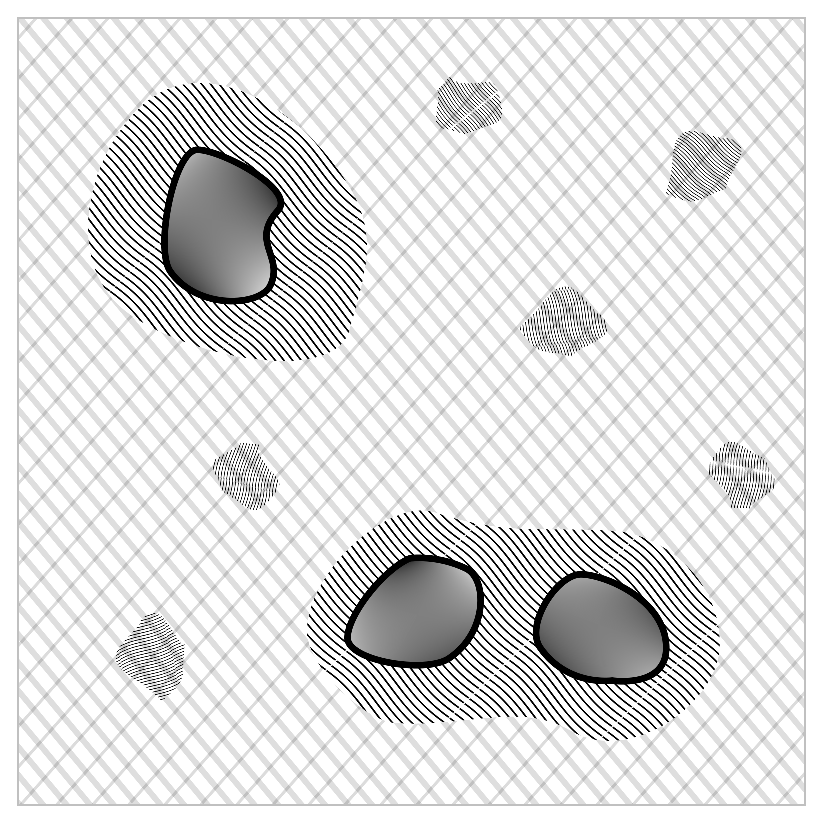
\includegraphics[width=0.45\textwidth]{images/PCE.eps}\quad
            \includegraphics[width=0.45\textwidth]{images/PEO-OMPEO.eps}};
            \begin{scope}[x={(image.south east)},y={(image.north west)}]
                % \draw[red, very thick] (0.49,0.69) ellipse (0.08 and 0.05);
                % \draw[red, very thick] (0.6,0.72) ellipse (0.07 and 0.3);
                % \draw[red, very thick] (0.75,0.67) ellipse (0.12 and 0.06);
                \draw[->, thick] (0.18,0.1) -- (0.25,0.2);
                \draw[->, thick] (0.22,0.1) -- (0.35,0.2);
                \draw[->, thick] (0.16,0.1) -- (0.12,0.68);
                \node[] at (0.2,0.05) {Polymer blends};
                \draw[->, thick] (0.3,0.5) -- (0.18,0.62);
                \draw[->, thick] (0.31,0.37) -- (0.32,0.32);
                \node[] at (0.32,0.47) {Області аморфізованого};
                \node[] at (0.25,0.41) {полімеру};
                \draw[->, thick] (0.37,0.9) -- (0.42,0.83);
                \draw[->, thick] (0.35,0.9) -- (0.33,0.63);
                \node[] at (0.35,0.95) {Полімерні кристаліти};
            \end{scope}
\end{tikzpicture}

% \begin{figure}
%           \begin{center}
%             \begin{overpic}[width=0.4\textwidth]{images/PCE.eps}
%                  \put(2,40){polymer blends}
%                  \put(2,40){amorphous regions}
%                  \put(2,40){small polymer crystalytes}
%             \end{overpic}
%             \quad
%             \begin{overpic}[width=0.45\textwidth]{images/PEO-OMPEO.eps}
%                  %\put(2,40){$\cal{D}$}
%             \end{overpic}
%           \end{center}
% \end{figure}
\end{document}